\documentclass{beamer}



%\usepackage{beamerthemesplit}
\usetheme{Boadilla}
%\usetheme{default}
%\useinnertheme{rounded}

%\useoutertheme{shadow}
\usecolortheme{rose}
%\usefonttheme{serif}
\setbeamertemplate{navigation symbols}{}
\usetheme{Madrid}

\usepackage{amssymb,amsmath,amscd,amsfonts,amsthm,dsfont,color,graphicx}
\usepackage{amscd}
%\usepackage[numbers]{natbib}
% \usepackage[french]{babel}
%\usepackage[active]{srcltx}


\def\qd{\,{\mathchar'26\mkern-12mu d}}

% \date[]{}

 \newcommand\makebeamertitle{\frame{\maketitle}}%

 \AtBeginDocument{
   \let\origtableofcontents=\tableofcontents
   \def\tableofcontents{\@ifnextchar[{\origtableofcontents}{\gobbletableofcontents}}
   \def\gobbletableofcontents#1{\origtableofcontents}
 }
\numberwithin{equation}{section}
  \theoremstyle{plain}
  \newtheorem*{thm*}{\protect\theoremname}
  \theoremstyle{plain}
  \newtheorem*{cor*}{\protect\corollaryname}
 \theoremstyle{definition}
 \newtheorem*{defn*}{\protect\definitionname}
 \theoremstyle{plain}
\newtheorem*{lem*}{\protect\lemmaname}
  \theoremstyle{plain}
  \newtheorem*{rem*}{\protect\remarkname}
   \theoremstyle{definition}
 \newtheorem*{prop*}{\protect\propositionname}

\usetheme{Madrid}

\makeatother

  \providecommand{\corollaryname}{Corollary}
  \providecommand{\definitionname}{Definitioninition}
  \providecommand{\theoremname}{Theorem}
   \providecommand{\lemmaname}{Lemma}
   \providecommand{\remarkname}{Remark}
   \providecommand{\propositionname}{Proposition}
   
   
\newcommand{\Rl}{\mathbb{R}}
\newcommand{\Cplx}{\mathbb{C}}
\newcommand{\Itgr}{\mathbb{Z}}
\newcommand{\Ntrl}{\mathbb{N}}
\newcommand{\Circ}{\mathbb{T}}
\newcommand{\Sb}{\mathbb{S}}
\newcommand{\Disc}{\mathbb{D}}
\newcommand{\Aff}{\mathbb{A}}

% The Caligraphic alphabet
\newcommand{\Ac}{\mathcal{A}}
\newcommand{\Bc}{\mathcal{B}}
\newcommand{\Cc}{\mathcal{C}}
\newcommand{\Dc}{\mathcal{D}}
\newcommand{\Ec}{\mathcal{E}}
\newcommand{\Fc}{\mathcal{F}}
\newcommand{\Gc}{\mathcal{G}}
\newcommand{\Hc}{\mathcal{H}}
\newcommand{\Ic}{\mathcal{I}}
\newcommand{\Jc}{\mathcal{J}}
\newcommand{\Kc}{\mathcal{K}}
\newcommand{\Lc}{\mathcal{L}}
\newcommand{\Mv}{\mathcal{M}}
\newcommand{\Nv}{\mathcal{N}}
\newcommand{\Oc}{\mathcal{O}}
\newcommand{\Pc}{\mathcal{P}}
\newcommand{\Qc}{\mathcal{Q}}
\newcommand{\Rc}{\mathcal{R}}
\newcommand{\Sc}{\mathcal{S}}
\newcommand{\Tc}{\mathcal{T}}
\newcommand{\Uc}{\mathcal{U}}
\newcommand{\Vc}{\mathcal{V}}
\newcommand{\Wc}{\mathcal{W}}
\newcommand{\Xc}{\mathcal{X}}
\newcommand{\Yc}{\mathcal{Y}}
\newcommand{\Zc}{\mathcal{Z}}


\newcommand{\Sp}{\mathrm{Sp}}
\newcommand{\tr}{\mathrm{tr}}
\newcommand{\Op}{\mathrm{Op}}
\newcommand{\sym}{\mathrm{sym}}
\newcommand{\Vol}{\mathrm{Vol}}
\newcommand{\Tr}{\mathrm{Tr}}
\newcommand{\dist}{\mathrm{dist}}
\newcommand{\sgn}{\operatorname{sgn}}
\newcommand{\diag}{\mathrm{diag}}
\newcommand{\id}{\mathrm{id}}
\newcommand{\Poly}{\mathrm{Poly}}

\newcommand{\spec}{\mathrm{Spec}}
\newcommand{\abs}{\mathrm{abs}}

\newcommand{\CV}{\mathrm{CV}}
\newcommand{\PCV}{\mathrm{PCV}}


% Used for highlighting. To remove all highlighting just make the command blank
\newcommand{\hl}{\color{red}}



\newcommand{\dom}{\mathrm{dom}}
\newcommand{\Bl}{\mathbb{B}^4}
\newcommand{\supp}{\mathrm{supp}}
\newcommand{\BS}{\mathfrak{BS}}
\newcommand{\dyad}{\mathrm{dyad}}
\newcommand{\Qs}{\mathscr{Q}}
\newcommand{\Av}{\mathrm{Av}}
\newcommand{\loc}{\mathrm{loc}}
% DOI transformer
\newcommand{\Ti}{\mathcal{T}}
\newcommand{\sa}{\mathrm{sa}}

\newcommand{\mf}{\mathfrak{m}}

\newcommand{\gf}{\mathfrak{g}}
\newcommand{\tf}{\mathfrak{t}}

\newcommand{\Str}{\operatorname{Str}}
   
\begin{document}

\title[Weyl law and the tangent groupoid]{Dave-Haller's Weyl law and the tangent groupoid}


\author[E. McDonald]{Edward McDonald (Penn State University)}


\institute[]{\tiny{University of Wollongong} }

\makebeamertitle


\begin{frame}{Introduction}
  This talk is based on none of my own work, instead I want to advertise the following two papers:
  \begin{center}
    E.~Van Erp and R.~Yuncken, A groupoid approach to pseudodifferential calculi. \emph{J. Reine Angew. Math.} \textbf{756} (2019), 151--182.
  \end{center}
  and
  \begin{center}
    S.~Dave and S.~Haller, The heat asymptotics on filtered manifolds \emph{J. Geom. Anal.} \textbf{30} (2020), no. 1, 337--389.
  \end{center}
\end{frame}

\begin{frame}{Plan for this talk}
    \begin{enumerate}
        \item{} Carnot-Caratheodory geometry
        \item{} The tangent groupoid (of Connes)
        \item{} The $H$-tangent groupoid (of van Erp and Yuncken)
        \item{} The Volterra calculus
        \item{} Dave-Haller's Weyl law for $H$-elliptic operators.
    \end{enumerate}
\end{frame}

\begin{frame}{Asteroids}
  In the classic game of asteroids, a player controls a spaceship moving on a two dimensional toroidal space, $\Rl/\Itgr\times \Rl/\Itgr.$ There are two controls available:
  \begin{enumerate}[{\rm (i)}]
    \item{} The spaceship can be rotated,
    \item{} The spaceship can be moved forward.
  \end{enumerate}
\end{frame}


\begin{frame}{Asteroids}
  The configuration space of the game is the three-dimensional torus $\Circ^3 = (\Rl/\Itgr)^3,$ with coordinates $(x,y,\theta),$ where $(x,y)$ is the position of the spaceship and $\theta$ is its angle.

  The controls of the game allow us to move along the vector fields
  \[
    X = \cos(\theta)\partial_x+\sin(\theta)\partial_y,\quad Y = \partial_\theta.
  \]
  \pause
  The player moves the spaceship along a path which is parallel to the span of $X$ and $Y.$ That is, the path of the spaceship in configuration space is $\{\gamma(t)\}_{t\geq 0},$ where
  \[
    \dot{\gamma}(t) \in \mathrm{span}\{X_{\gamma(t)},Y_{\gamma(t)}\},\quad t\geq 0.
  \]
  \pause
  Despite there being only two available directions, we can reach any point $(x,y,\theta)$ from any other point by travelling parallel to $X$ and $Y.$
\end{frame}


\begin{frame}{Asteroids}
  A random walk making independent increments in the $X$ and $Y$ directions looks a bit like this:
  \begin{center}
  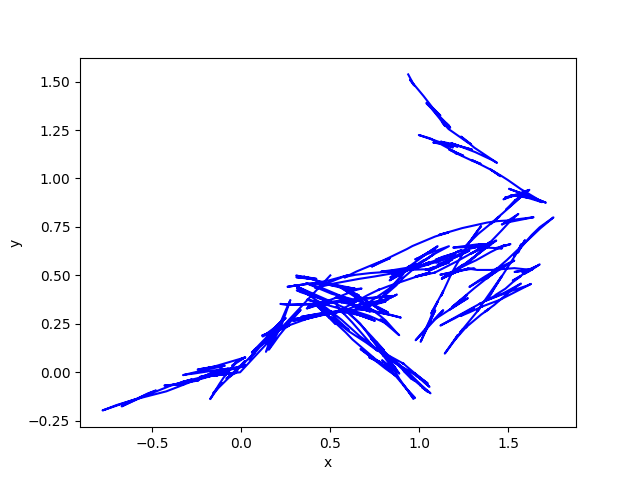
\includegraphics[width=90mm]{xy_coords_single_paths.png}
  \end{center}
  (this is displayed in ``unwrapped" coordinates, i.e. we do not take the quotient modulo $\Itgr.$).
\end{frame}

\begin{frame}{Asteroids}
  Ten realisations of the same random walk look like this:
  \begin{center}
    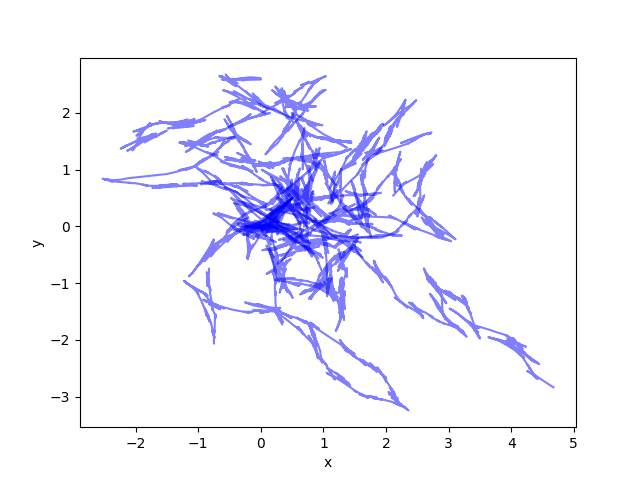
\includegraphics[width=90mm]{xy_coords_multiple_paths.png}
  \end{center}
\end{frame}

\begin{frame}{Asteroids}
  The real path through configuration space is in three dimensions, and looks like this:
  \begin{center}
  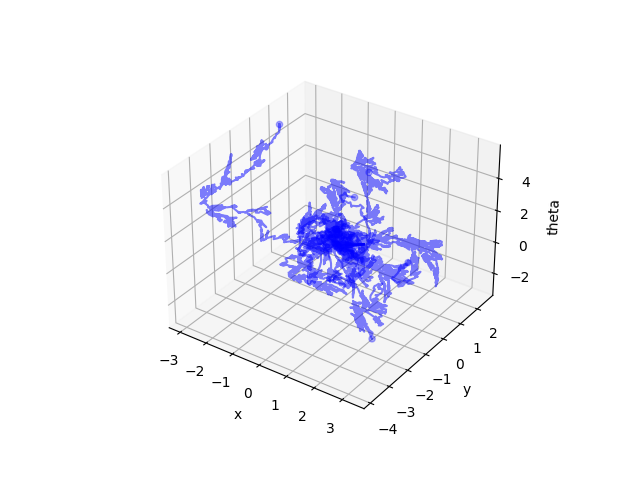
\includegraphics[width=90mm]{xyt_coords_multiple_paths.png}
  \end{center}
\end{frame}


\begin{frame}{Asteroids}
  In general, if we can travel parallel to $X$ and $Y$ then we can approximate paths along $[X,Y],$ by the Lie-Kato-Trotter product formula
  \[
    \exp(t[X,Y]) = \lim_{n\to\infty} (\exp(\frac{t}{n}X)\exp(\frac{t}{n}Y)\exp(-\frac{t}{n}(X+Y))\exp(-\frac{t}{n}Y))^n.
  \]
  But moving along $[X,Y]$ is harder than moving along $X$ and $Y.$

  In the asteroids example,
  \[
    [X,Y] = \sin(\theta)\partial_x-\cos(\theta)\partial_y
  \]
  so $\{X,Y,[X,Y]\}$ form a basis for the tangent space to $\Circ^3$ at every point.
\end{frame}

\begin{frame}{Asteroids}
  Thinking about $X$ and $Y$ as derivations (not just as directions), we should think of $X,Y$ as being order $1$ and $[X,Y]$ as being order $2.$

  The operator
  \[
    \Theta = X^2+Y^2 = \partial_\theta^2+(\cos(\theta)\partial_x+\sin(\theta)\partial_y)^2
  \]
  is homogeneous of order $2.$
  \pause
  \begin{itemize}
    \item{} $\Theta$ is not elliptic, but $(1-\Theta)^{-1}$ does improve regularity somewhat. Why, and by how much?
    \item{} The spectrum of $\Theta$ is discrete, with a sequence of eigenvalues $0\leq \lambda(1,-\Theta) \leq \lambda(2,-\Theta) \leq \cdots$ What is their asymptotic behaviour?
  \end{itemize}
\end{frame}

\begin{frame}{Asteroids}
 Let $\|u\|_{s}$ denote the standard Hilbert-Sobolev norm of order $s$ of $u\in C^\infty(\Circ^3).$ That is,
 \[
      \|u\|_s := \|(1-\partial_x^2-\partial_y^2-\partial_z^2)^{\frac{s}{2}}u\|_{L_2(\Circ^3)}.
 \]
 A highly non-trivial calculation gives us the \emph{sub-elliptic estimates}:
  \[
      \|u\|_{s+\frac12}\lesssim_s \|\Theta u\|_s+\|u\|_s.
  \]
  This implies hypoellipticity (i.e., $\Theta u\in C^\infty \Rightarrow u \in C^\infty$) and also the discreteness of the spectrum of $\Theta.$
\end{frame}

\begin{frame}
  It is not obvious at all, but
  \[
    \lambda(n,-\Theta) \sim \frac{2\sqrt{3}}{\pi} n^{\frac{1}{2}},\quad n\to\infty
  \]
  Note that an elliptic second order operator $P\geq 0$ on a compact $d$-manifold $X$ obeys
  \[
    \lambda(n,P) \sim c_d n^{\frac{2}{d}}.
  \]
  \emph{The spectral dimension of Asteroids is $4$, not three!}
  \pause
  What is going on here?
\end{frame}

\begin{frame}{Carnot manifolds}
  The plane bundle $\mathrm{span}(X,Y)\subset T\Circ^3$ is an example of a contact structure, and this leads us to what is in general called a Carnot manifold.
  \begin{definition}
    A \emph{Carnot manifold} is a manifold $X$ equipped with a filtration of sub-bundles of $TX.$ That is, there are subbundles $(H^j)_{j=0}^N$ such that
    \[
      0 = H^0 < H^1 < \cdots < H^N = TX
    \]
    and if $E\in \Gamma H^j, F\in \Gamma H^j,$ then $[E,F] \in \Gamma H^{j+k}.$
  \end{definition}
  We should think of the directions in $H^j$ as having ``order $j$".
  \pause
  I will concentrate on the example $X = \Circ^3,$ with $N=2$ and $H^1 = \mathrm{span}\{X,Y\}.$
\end{frame}


\begin{frame}{Graded Lie groups}
  The most fundamental example of a Carnot manifold is a graded nilpotent Lie group. These are important in the general theory as local models.

  Let $\gf$ be a Lie algebra which admits a direct sum decomposition
  \[
    \gf = \bigoplus_{n=1}^\infty \gf_n
  \]
  where $[\gf_k,\gf_n] \subseteq \gf_{k+n}.$ This is called a stratified Lie algebra. Being finite dimensional, it is easy to see that $\gf$ is nilpotent.

  The number
  \[
    Q := \sum_{n=1}^\infty n\mathrm{dim}(\gf_n)
  \]
  is called the homogeneous dimension of $\gf.$
\end{frame}

\begin{frame}{Graded Lie groups}
  Exponentiating $\gf,$ we get a simply connected Lie group
  \[
    G = \exp(\gf).
  \]
  Nilpotent groups are very special: the exponential mapping is a homeomorphism, and the Lebesgue measure of $\gf$ pushes forward to the Haar measure of $G.$
%   Suppose that $\gf_1$ has a basis $\{X_1,\ldots,X_m\}.$ Under the homeomorphism $G\approx \Rl^N,$ the basis
%   \[
%     X_1,\ldots,X_m
%   \]
%   is a family of vector fields with polynomial coefficients satisfying the H\"ormander condition at every point.
\end{frame}


\begin{frame}{Graded Lie groups}
  The prototypical example is the Heisenberg Lie group. This one has $\gf = \mathrm{span}\{\Xc,\Yc,\Tc\},$ with $[\Xc,\Yc] = \Tc$ and all other commutators vanishing. The grading is
  \[
    \gf_1 = \mathrm{span}\{\Xc,\Yc\},\quad \gf_2 = \mathrm{span}\{\Tc\}.
  \]
\end{frame}

\begin{frame}{The osculating group}
  From the data of $(X,H),$ we define the {\it associated graded bundle} $\mathfrak{t}_HX$, which is the graded vector bundle over $X$ formed by
  \[
      \mathfrak{t}_HX=\bigoplus_{n=1}^N (\mathfrak{t}_HX)^n,\qquad\text{where}\qquad (\mathfrak{t}_HX)^n=H^n/H^{n-1}.
  \]
  If $X\in\Gamma (\mathfrak{t}_HX)^n$, and $Y\in \Gamma(\mathfrak{t}_HX)^m$, then
  $[X,Y]$ is a well-defined section of $(\mathfrak{t}_HX)^{n+m}$. Here, $\Gamma E$ denotes the space of smooth sections of a vector bundle $E.$ In fact more is true, for smooth functions $f,g$, we then have
  \[
      [fX,gY]-fg[X,Y]\in\Gamma H^{n+m-1}.
  \]
  This implies that the commutator of vector fields descends to a Lie bracket on the the fibres of $\tf_HX.$ That is, $\tf_HX$ is a bundle of graded nilpotent Lie groups.

  The fibrewise exponential $T_HX := \exp(\tf_HX)$ is called the \emph{osculating group} of the filtration $H.$

  \pause
  We should think of the $T_HX$ as being an infinitesimal model for $X$ with its filtration $H.$
\end{frame}

\begin{frame}{The Connes tangent groupoid}
  The usual recipe for defining pseudodifferential operators on a manifold $X$ is the following procedure:
  \begin{enumerate}
      \item{} Identify a class of symbols $\sigma$ on $\Rl^d.$
      \item{} Define pseudodifferential operators $\Op(\sigma)$ by a quantisation formula such as
      \[
        \Op(\sigma)u(x) = (2\pi)^{-d} \int_{\Rl^d} e^{i(x,\xi)} \sigma(x,\xi)\widehat{f}(\xi)\,d\xi
      \]
      \item{} Show that the class of pseudodifferential operators just defined is invariant under change of variables
      \item{} A pseudodifferential operator on a manifold $X$ is a linear operator $T:C^\infty_c(X)\to C^\infty(X)$ which has smooth kernel away from the diagonal and which is pseudodifferential in every chart.
  \end{enumerate}
  This is a little inelegant, is there a better way?
\end{frame}

\begin{frame}{Semiclassical quantisation}
  Often it is better to quantise a symbol $\sigma$ into a whole family of operators $\Op_{\hbar}(\sigma)$ depending on a parameter $\hbar,$ by a formula such as
  \[
    \Op_{\hbar}(\sigma)u(x) = (2\pi)^{-d} \int_{\Rl^d} e^{i(x,\xi)}\sigma(x,\hbar \xi)\widehat{f}(\xi)\,d\xi.
  \]
  As $\hbar\to 0,$ the noncommutative algebra of $\hbar$-pseudodifferential operators under operator composition is supposed to reduce to the commutative algebra of symbols under pointwise multiplication.
\end{frame}


\begin{frame}{Kernels of pseudodifferential operators}
  The Schwartz kernel of a pseudodifferential operators with symbol $\sigma$ is given by the oscillatory integral
  \[
      K(x,y) = (2\pi)^{-d}\int_{\Rl^d} e^{i(x-y)\cdot \xi}\sigma(x,\xi)\,d\xi
  \]
  (in the distribution sense). If we consider the kernel $K(\cdot,\cdot,\hbar)$ of the $\hbar$-quantisation, we should have
  \[
      K(x,y,\hbar) = (2\pi \hbar)^{-d} \int_{\Rl^d} e^{i\frac{x-y}{\hbar}\cdot \xi}\sigma(x,\xi)\,d\xi.
  \]
  In the limit as $\hbar\to 0,$ what should happen is that this looks more and more like the kernel of a convolution operator.
  Really, the kernel $K$ of a pseudodifferential operator on a manifold $X$ should be thought of as a function (distribution) on the space
  \[
      \mathbb{T}X = (TX\times \{0\})\sqcup (X\times X\times (0,\infty)).
  \]
\end{frame}

\begin{frame}{The tangent groupoid}
  Let $X$ be a manifold, and define the set
  \[
    \mathbb{T}X = (TX\times \{0\})\sqcup (X\times X\times \Rl^{\times}).
  \]
  Connes invented a good topology for $\mathbb{T}X,$ making it a manifold of dimension $2\mathrm{dim}(X)+1.$ Better yet, this is a \emph{Lie groupoid}, with range and source maps
  \[
    r(x,y,\hbar) = (x,\hbar),\quad s(x,y,\hbar) = (y,\hbar),\quad r((x,z),0) = s((x,z),0) = (x,0)
  \]
  and composition law
  \[
    (x,y,\hbar)\circ (y,w,\hbar) = (x,w,\hbar),\quad ((x,z),0)\circ ((x,z'),0) = (x,z+z',0).
  \]
\end{frame}

\begin{frame}{The tangent groupoid}
  Elements of the convolution algebra of the groupoid $\mathbb{T}X$ are distributions $f,g \in \Dc'(\mathbb{T}X),$ with convolution product
  \[
    (f\ast g)(x,y,h) = \int_{X} f(x,w,h)g(w,y,h)\,dw,\quad (f\ast g)((x,z),0) =\int_{T_xX} f((x,z-z'),0)g((x,z'),0)\,dz'.
  \]
  That is: the convolution of distributions on $\mathbb{T}X$ looks like composition of kernels of pseudodifferential operators.

  Can we use this as a basis to define an algebra of pseudodifferential operators?
\end{frame}


\begin{frame}{The zoom action}

\end{frame}




\begin{frame}
\structure{\begin{center}
{\Huge{}Thank you for listening!}
\par\end{center}}\end{frame}



\end{document}

